
\begin{frame}{Introduction}
  \begin{block}{Current Many-Core Architectures}
    \begin{itemize}
     \item High FLOP/Watt ratio
     \item High memory bandwidth
     \item Attached via PCI-Express
    \end{itemize}
\vspace*{1cm}
  \end{block}

   \begin{minipage}{0.3\textwidth}
    \begin{center}
     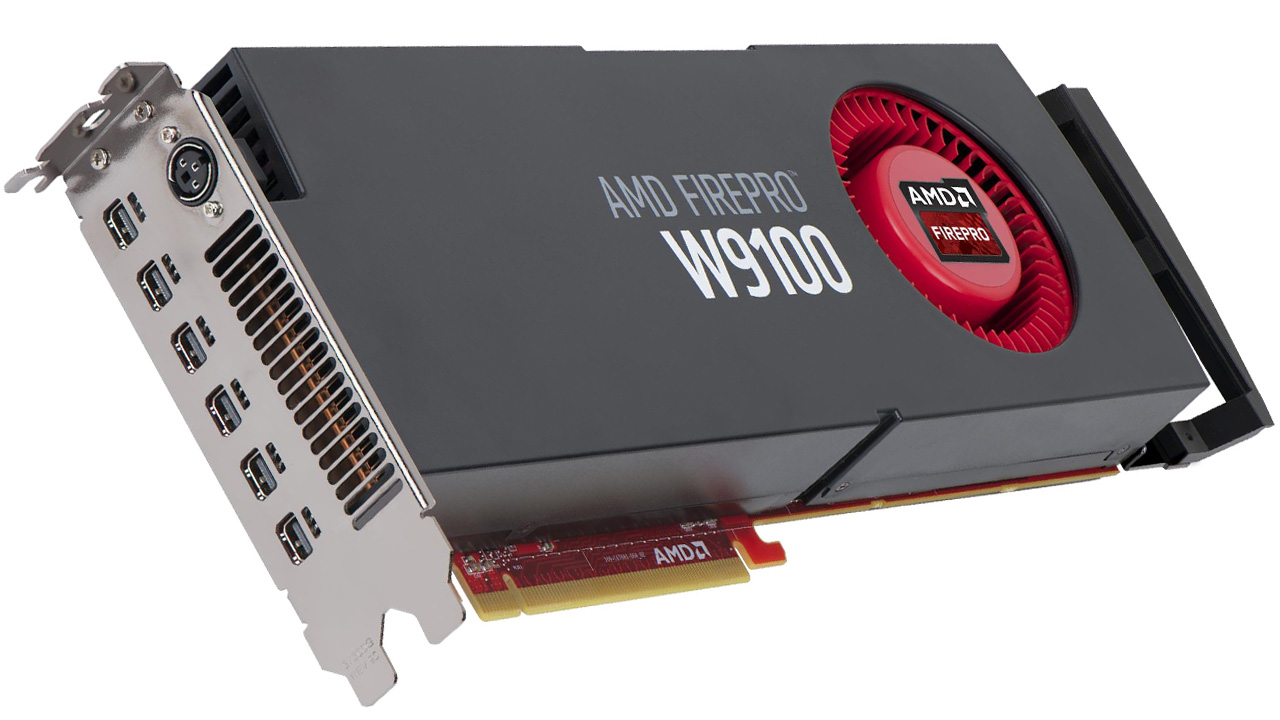
\includegraphics[width=0.99\textwidth]{figures/w9100.jpg} \\ AMD FirePro W9100 \\ 320 GB/sec
    \end{center}
   \end{minipage}
   \hspace{0.2cm}
%
   \begin{minipage}{0.3\textwidth}
    \begin{center}
     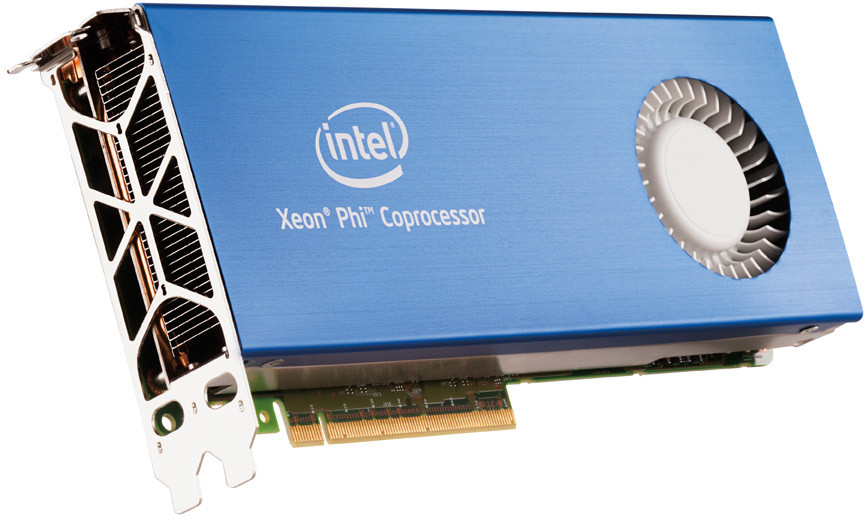
\includegraphics[width=0.92\textwidth]{figures/xeon-phi.jpg} \\ INTEL Xeon Phi \\ 320 (220?) GB/sec
    \end{center}
   \end{minipage}
   \hspace{0.2cm}
%
   \begin{minipage}{0.3\textwidth}
    \begin{center}
     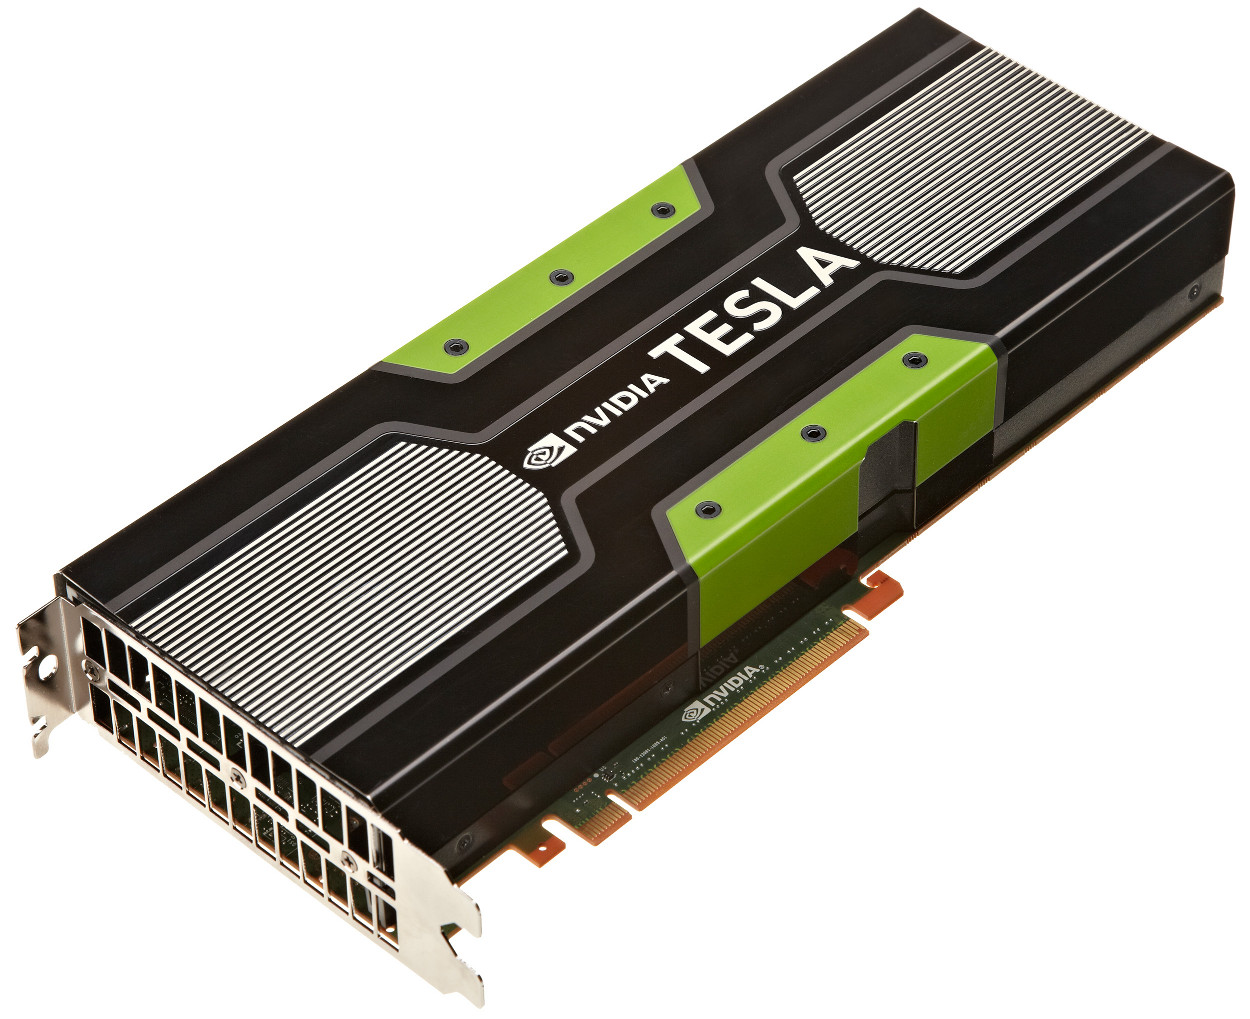
\includegraphics[width=0.7\textwidth]{figures/TeslaK20.jpg} \\ NVIDIA Tesla K20 \\ 250 (208) GB/sec
    \end{center}
   \end{minipage}


\end{frame}


\begin{frame}{Introduction}
 \vspace*{-0.5cm}
 \begin{center}
  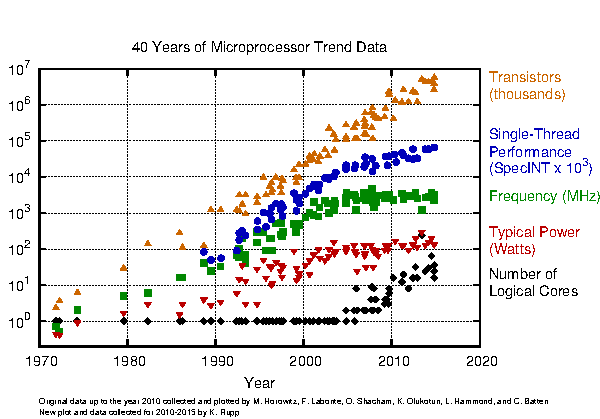
\includegraphics[width=0.95\textwidth]{figures/40-years-processor-trend}
 \end{center}
 {\tiny https://www.karlrupp.net/2015/06/40-years-of-microprocessor-trend-data/ }
\end{frame}

\begin{frame}{Introduction}
 \vspace*{-0.5cm}
 \begin{center}
  Theoretical Peak Performance \\
  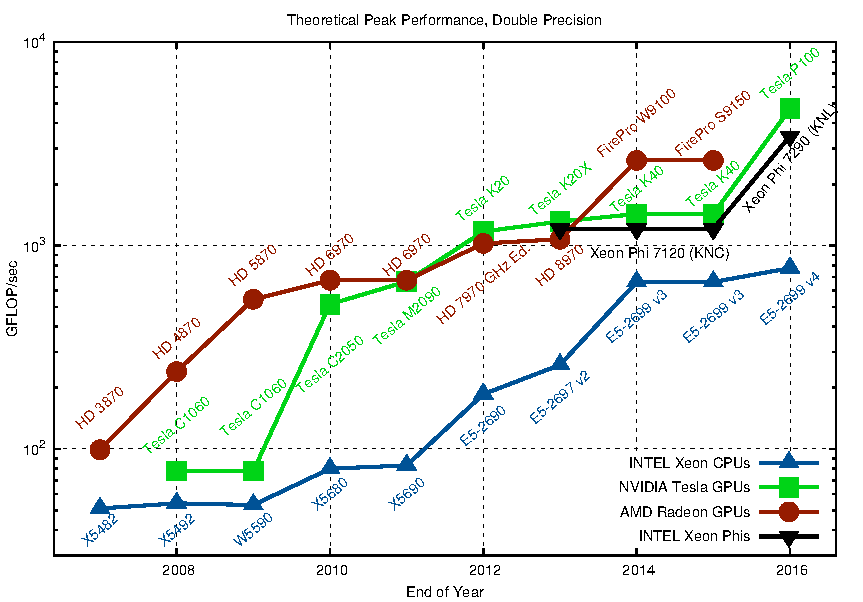
\includegraphics[width=0.95\textwidth]{figures/gflops-dp}
 \end{center}
 \vspace*{-0.5cm}
 {\tiny https://www.karlrupp.net/2013/06/cpu-gpu-and-mic-hardware-characteristics-over-time/ }
\end{frame}

\begin{frame}{Introduction}
 \vspace*{-0.5cm}
 \begin{center}
  Theoretical Peak Performance per Watt \\
  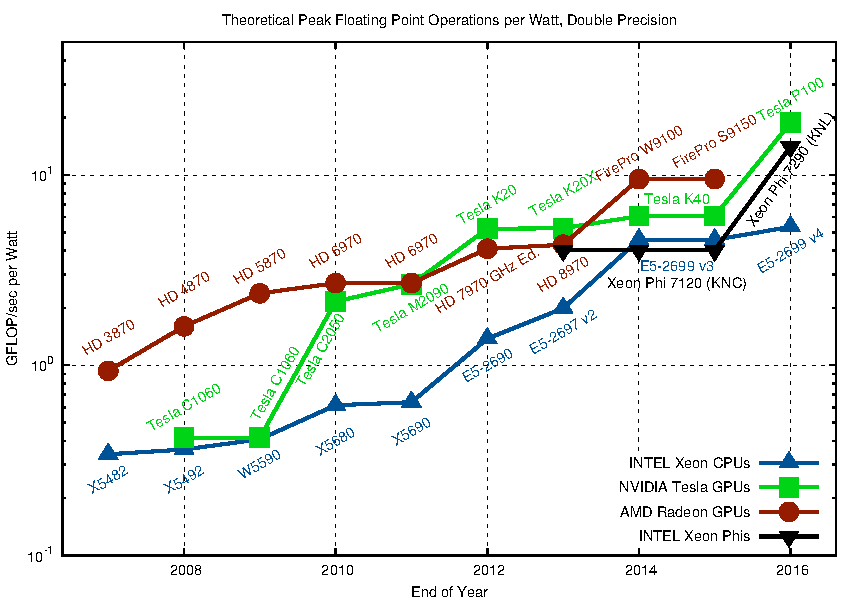
\includegraphics[width=0.95\textwidth]{figures/gflops-per-watt-dp}
 \end{center}
 \vspace*{-0.5cm}
 {\tiny https://www.karlrupp.net/2013/06/cpu-gpu-and-mic-hardware-characteristics-over-time/ }
\end{frame}

\begin{frame}{Introduction}
 \vspace*{-0.5cm}
 \begin{center}
  Theoretical Peak Performance (FLOPs) per Byte of Memory Bandwidth \\
  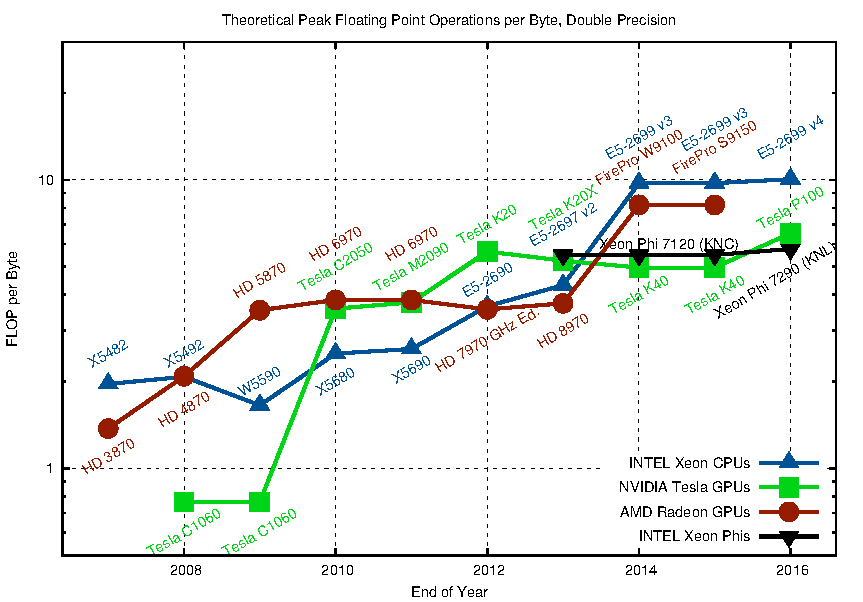
\includegraphics[width=0.95\textwidth]{figures/flop-per-byte-dp}
 \end{center}
 \vspace*{-0.5cm}
 {\tiny https://www.karlrupp.net/2013/06/cpu-gpu-and-mic-hardware-characteristics-over-time/ }
\end{frame}



